\documentclass[ author={Stephen Livermore-Tozer},
				supervisor={Dr. Peter Flach},
				degree={MEng},
				title={Performing Algorithmic Co-composition Using Machine Learning},
				subtitle={},
				type={research},
				year={2016} ]{dissertation}
				
\usepackage{tikz}
\usetikzlibrary{matrix,chains,positioning,decorations.pathreplacing,arrows}
\usepackage{graphicx}
\usepackage{hyperref}

%\renewcommand{\baselinestretch}{1.15} 

\DeclareMathOperator*{\argmin}{arg\,min}
\DeclareMathOperator*{\argmax}{arg\,max}

\begin{document}
	
	\maketitle
	
	\frontmatter
	
	\makedecl
	
	\tableofcontents
	\lstlistoflistings
	
	% -----------------------------------------------------------------------------
	
	\chapter*{Executive Summary}
	
	% Hypothesis
	For my research, I have investigated the hypothesis that existing methods of performing melodic composition using machine learning can be adapted to successfully perform co-composition with a human composer. In this context, success may be measured by subjective impression received from experts in composition. The exact set of tasks involved in the co-composition process is not fixed; part of this research involved finding the tasks that are both a) useful to the composer, and b) within the capabilities of current AI.
	
	% Achievements
	In the pursuit of this objective, I have completed the following tasks:
	\begin{itemize}
		\item I surveyed a number of expert composers to identify the tasks within the domain of composition whose partial automation would provide the greatest benefit to the composer.
		\item I performed research over existing machine learning methods for algorithmic composition, determining their applicability and estimated efficacy within the tasks obtained above.
		\item I implemented an application that may be trained on a set of music data (stored in the Midi format) and will provide an attempted continuation of a given musical input, according to the tasks obtained above.
		\item I designed and performed a series of objective and subjective tests to assess the performance of the application and the algorithms that comprise it.
	\end{itemize}
	
	
	% -----------------------------------------------------------------------------
	
	\chapter*{Supporting Technologies}
	
	I used the Anaconda implementation of Python included with the Spyder IDE to create my application. Furthermore, I used a set of libraries implementing utilities and machine learning techniques to create the application. These libraries are: 
	
	\begin{itemize}
		\item Mido for Midi file processing
		\item NumPy for efficient mathematical operations
		\item SciPy for clustering and regression
		\item PyBrain for neural networks
		\item HmmLearn for hidden Markov models
	\end{itemize}
	
	% -----------------------------------------------------------------------------
	
	\chapter*{Acknowledgements}
	
	I would like to thank my supervisor Peter Flach for his guidance over the course of this project in both its technical aspects and in its effective management.
	
	\mainmatter
	
	% -----------------------------------------------------------------------------
	
	\chapter{Contextual Background}
	\label{chap:context}
	
	\section{Overview}
	
	Algorithmic composition is an AI problem concerning the creation of music via some algorithmic process. It is currently one of the topics at the forefront of the greater study of \textit{computational creativity}: the challenge of designing an AI that displays, according to some agreeable definition, creativity. This can be described in another way as algorithmically mimicking various aspects of human intelligence, particularly relating to the conception of novel solutions to problems. The arts are a particular subject of interest for this research, as they are widely considered to be highly creative and distinctly human.
	
	From an AI researcher's perspective, algorithmic composition is not too different in some ways from most other AI tasks: the goal is to design an algorithm that can analyse some complex natural process, derive an abstract model from the available data, and then select actions according to that model. The subject being modelled in this instance however is a psychological process that is both difficult to measure and relatively poorly understood. Many attempts have been made to find an effective way to deal with this problem; some have attempted a bottom-up approach based directly on human psychology, some have attempted to build a top-down model based on known musical principles, and yet others have tried to tackle it as a purely data-oriented task.

	\section{Computational Creativity}
	
	%TODO: Maybe move Machine Learning (ML) to the acronyms section?
	Artificial intelligence as a field has grown a great deal from its first appearance on the academic landscape 60 years ago. It has suffered a fairly shaky history, rising and falling from prominence several times throughout its short life thus far, before reaching its current widespread mainstream adoption and high value in industrial application. Currently techniques that form a part of AI, such as machine learning (ML), are used in a huge number of environments to tackle a wide range of problems. It has become apparent that almost any area in which data analysis plays a large role is a viable target for AI intervention. This not only targets traditional data-heavy fields such as marketing or economics, but also enables complex tasks such as processing natural language, bioinformatics, and autonomous robotic locomotion. While growth and decline is not unknown to AI, it currently occupies a major role in the modern technological landscape and does not show any immediate signs of slowing.
	
	Furthermore, the influence of AI spreads beyond the direct technological applications alone. Even since before the formalization of AI as a field, there has existed a cultural fascination with the concept of intelligent machines. There has been much speculation about the ethical and philosophical implications of the creation of an intelligent mind, and a great deal of fiction has been created with the topic as a central theme. In more recent times as AI has become widely prominent, new hopes and worries have begun to emerge with regards to the social impact, ethical impact, and potential dangers of advanced AI systems. It is in this context that the ultimate capabilities of modern AI technology has fallen into sharp focus.
	
	Currently, the greatest weakness of AI is seen to be in displaying human-like creativity. Although AI is very powerful within domains that have been sufficiently well formalized, there are many fields that remain substantially informal. The most significant of these are the arts. Machines have, to this day, failed to demonstrate any artistic merit of significance that approaches the level of a skilled human. While AI has demonstrated a certain degree of proficiency at specific well-defined tasks within artistic subjects, such as identifying artists from their paintings \cite{blessing2010using} or genres of music \cite{haggblade2011music}, AI remains unable to perform broader creative tasks such as creating or appraising art in a human-like fashion. A good deal of research has been put towards tackling this identified weakness from the academic community, but despite occasional novel results overall progress is proving slow. This deficiency is exacerbated to no small degree by the fact that there is little overlap otherwise between AI and the arts, making it difficult for collaboration or the sharing of knowledge and results between the two.
	
	
	\section{Algorithmic Composition}
	
	One of the areas of artificial creativity currently under focus is algorithmic composition. Algorithmic composition is the general term for the application of algorithms in some form to the task of musical composition - in short, AI that can write music. This is a particularly enticing challenge for those interested in artificial creativity, as music is generally considered to be the most mathematical of all the arts. Various aspects of music at both the physical and compositional level exhibit a very strong degree of structure that can be described mathematically, and conversely elements of mathematics have been directly employed by composers in the creation of their work. This provides a strong argument for music as one of the best suited art forms for analysis by AI, as musical data may be meaningfully digested computationally and consists of patterns and structures that may apparently be learned and predicted. 
	
	%TODO: Give examples of AI-composed music
	In practice however, AI still has a long way to go. Much exploration has been made with the goal of finding an algorithm that produces satisfactory results, but as of yet even the most state of the art musical AIs have clear flaws and limitations. Most ``successful'' AI is specialized for a specific region of composition; common choices include harmonization \cite{freitas2011melody}, jazz improvisation \cite{franklin2001multi}, and full orchestral composition \cite{diaz2011composing}. The best performers within their respective regions produce work that is subjectively assessed as approximately equal to that of a novice composer. Most such work contains noticeable idiosyncrasies however, and despite being able to create amateur-level music the AI consistently fails to produce work comparable with that of skilled composers at even a small probability. This is generally attributed by both artists and certain AI specialists as a lack of creativity; although the AI is skilled at applying certain musical concepts effectively it does not feature the combination of novelty and coherency common to human work. This is not to say that AI as we currently know it is not capable of composition at a human-like level, but that current methods fall short of the mark.
	
	\subsection{Current Challenges}
	
	One of the unique challenges in computational creativity, particularly in algorithmic composition, is that it is very difficult to define creativity to begin with. In some circles of research the goal of computational creativity is in fact to simply understand human creativity in the first place. Because of this, setting an easily measurable objective for the creation of creative AI is implausible if not impossible; instead the metrics used to measure success are typically focused on subjective assessment, either by direct comparison with existing creative work or appraisal by trained art critics. One fairly scientific approach to this is the ``creative Turing test,'' a variant of the traditional Turing test in which a human subject converses through a terminal with both another human and a computer, without being informed which is which. The computer is considered to have passed the Turing test if the subject is unable to distinguish between the human and the computer through the conversation. This translates well into a test of creativity; a human may observe creative works produced by a computer and by a human, and attempt to distinguish which was created by the computer in the same manner. This can be a difficult test to pass depending on the particular creative medium being assessed. One important detail to note with regards to this challenge however is that it does not assess the subjective quality of the piece. This is very understandable given that subjective quality is difficult to define and cannot currently be measured computationally, but it nonetheless is one of the most important factors for any practical application of a creative AI.
	
	Beyond the more abstract difficulties involved however, there are significant technical challenges in replicating human-like musical composition. These include the compositional complexity of most musical pieces (even music considered relatively simple), the colossal variety of styles and genres of music in existence, and the difficulty in obtaining data relating to human appreciation of music. Most AI research thus far has primarily been concerned with creating a robust model for the complex patterns present in real music; typically the goal is either to imitate elements of a pre-specified corpus of music (as in \cite{paiement2007generative} \cite{todd1989connectionist}) or produce wholly original work according to some prior-defined style (\cite{diaz2011composing} \cite{burton1998hybrid} \cite{horowitz1995representing}). 
	
	Despite numerous attempts using a wide range of AI methods (described further in section \ref{sec:abstract-methods}) there have been few significant successes in achieving this goal. The most notable of these is Iamus, a supercomputer running software based on the Melomics system \cite{diaz2011composing}, and the first computer to compose professional contemporary classical music in its own style \cite{scientist2012computer}. This system used an evolutionary algorithm with manually-encoded rules as a fitness function (detailed in \ref{sec:hybrid-systems}), meaning that it was directly instructed on how to produce classical music without the need for any learning to take place. Iamus' work has received mixed critical reception, although there is the strong possibility of bias resulting from the fact that composer was already known by most critics to be a computer. Although this is a very impressive technical feat, it has not lead to any kind of industry adoption or significant public interest within the 6 years that have followed. This can be attributed to the fact that it exists as a standalone system; it does not integrate with any existing musical process and the work it produces is not in itself unique or useful.
	
	\section{Technology in Musical Composition}
	\label{sec:tech-in-music}
	
	As detailed above, there has been a substantial amount of work invested into algorithmic composition up to this point. It is of notable importance that the vast majority of this work has developed from academic interest only, with very little direct involvement from industry towards the problem (and many of the companies that are involved emerged directly from academia). The cause for this is easily identifiable: there are few current financial incentives to pursue algorithmic composition. Although a high quality artificial composer would certainly be a valuable asset, technology is recognizably quite far away from achieving something effective enough to put to market with a high expected return on investment. This slows down the rate of progress in the study of algorithmic composition, and quite possibly computational creativity as a whole; while current research is going strong, the problem being tackled is immense and the resources available comparatively small. 
	
	The financial incentive for investment in algorithmic composition given the reasonable possibility of achieving success is also quite evident. The music industry is currently valued at over \pounds 10.0 billion globally \cite{smirke2015global}, with the UK retail value worth over \pounds 900 million \cite{riaj2015global}. Any kind of new technology capable of providing a fundamental boon to production is therefore of high value. 
	
	% Traditional Composition stuff
	
	In modern times, technology has served to greatly augment the compositional process. The invention of the 
	analogue synthesizer and its subsequent rise to widespread popularity in the 1960s-1970s provided a powerful new tool to composers. This electronic instrument not only produced a unique sound unlike any traditional acoustic instruments, but proved highly versatile during composition due to the ability to synthesize sounds similar to different instruments. This functionality began to reach its true potential in the early 1980s, as polyphonic electronic keyboards incorporating many different sounds as part of their hardware began to enter popular use. This single piece of equipment gave individual producers the ability to both compose and perform each part of an entire multi-instrumental score by themselves. These advancements began to peak with the invention of software synthesizers and the MIDI format (see \ref{sec:midi}), imbuing a computer with the power to fully score and synthesize virtually any kind of music. These advances have had enormous consequences for the world of music, as it has become possible for any individual with access to an inexpensive digital workstation to create, perform, and distribute music that would have required an entire orchestra or even been impossible to create otherwise.
	
	% TODO: Definitely mention existing CAAC software (page 3 of the survey)
	
	\section{AI in Creative Media}
	
	Although artificial intelligence has enjoyed enormous recent success in research and industry, it has also begun to see employment in entertainment as well. Although no AI has yet taken over a popular, mainstream creative role ordinarily performed by humans, there have been many cases where an AI has provided novelty or entertainment within an established art form.
	
	\begin{figure}[h]
		\centering
		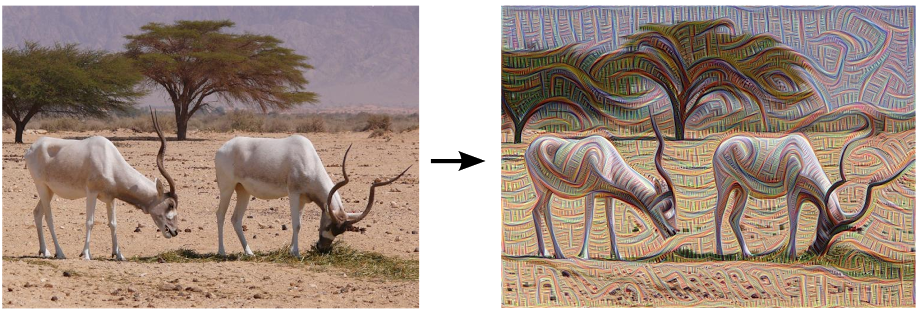
\includegraphics[width=1.0\textwidth]{deep-dream-example}
		\caption{An image before and after processing by Google DeepDream}
	\end{figure}
	
	One of the most recent well-known cases of this is Google's ``DeepDream,'' an online application that uses computer vision technology to enhance images according to detected features, morphing details to exaggerate falsely perceived visual elements (quite commonly biological) resulting in a highly surreal output reminiscent of dreams or hallucinations. This has received popular attention as potentially a form of true AI-created art, with numerous articles discussing the philosophical consideration that it could be considered true art \cite{rayner2016google} \cite{galperina2015google} and an actual art exhibition featuring its work \cite{campbell2016inside}.
	
	AI has also demonstrated a surprisingly high proficiency in writing both fiction and non-fiction. Technically-oriented AI writers have already been employed in a professional environment by the company Narrative Science, in the form of their Quill platform: a service that analyses data, identifies data trends and other kinds of useful information, and performs natural language communication to relay results and answer questions \cite{woodie2016big}. Creative AI has also seen recent success as an algorithmically co-written story was recently entered into a literary competition (intended primarily for humans) and outperformed many of its human competitors \cite{tarantola2016ai}. In this sense, computer-human collaboration has already reached the level of a skilled human within the domain of writing. 
	
	\section{Project Aims}
	
	The aim of this research project is to attempt to bridge some of the gap between the current theoretical state of algorithmic composition and the practical reality of AI in music. The final goal is the development of an algorithm that provides useful melodic material based on the work of a human composer in a manner that is realistic with regard to human composition.
	
	To be considered successful, this algorithm must demonstrate the ability to generate monophonic melodic music in a style that is similar to that of an existing musical piece. As the goal in this case is not to simply create an entire self-contained song but to assist a human in the creation of their own song, the algorithm should not simply output a single complete melody. Instead, the algorithm must be able to provide a set of different outputs for each position within the song so that utility to the user is maximized. Additional facilities to increase gain to the user, such as allowing the user to direct the generation process via some interactive means, are also being searched for. Finally, the program must be be such that regular use is feasible in a typical modern compositional context: there must be no hardware, time, or manpower requirements that would be extraordinary for a single musician working independently.
	
	To summarise, the specific objectives of this project are:
	\begin{enumerate}
		\item Survey literature relating to algorithmic melody composition to determine a set of viable methods for expanding existing musical scores
		\item Adapt one or more of these algorithms to write partial melodic sequences that fill gaps in or provide variations to an existing melody
		\item Implement an application using this algorithm that allows operation by a non-technical user in a timespan appropriate for practical use (a reasonable estimation would be 1 minute per bar)
		\item Assess the effectiveness of the algorithm(s) in the context of completing a melody through a set of objective tests
		\item Determine, for each algorithm being tested, a strategy that enables user interaction with the melodic generation process in some guiding capacity
		\item Assess the effectiveness of the extended algorithm(s) in the same manner as the original and determine the improvements offered by increased levels of human-computer interaction
	\end{enumerate}
	
	% -----------------------------------------------------------------------------
	
	\chapter{Technical Background}
	\label{chap:technical}
	
	This chapter covers previous work in the field of algorithmic composition, both as a broad overview of the landscape and an in-depth explanation of the particular work directly relevant to this research.

	\section{Abstract Methods for Algorithmic Composition}
	\label{sec:abstract-methods}
	
	Many common types of AI techniques have been used in some way for algorithmic composition. The majority of these techniques can be broadly categorised as one of:
	\begin{itemize}
		\item Knowledge-based models
		\item Supervised learning
		\item Evolutionary algorithms
		\item Hybrid models
	\end{itemize}
	Each of these categories carries their own set of advantages and disadvantages which greatly influence the type of output they produce. Although these categories are not restricted in the type of compositional tasks that they can perform, different techniques may result in completely different uses for the resulting AI. Examples of these different categories, some of the techniques that comprise them, and their strengths and weaknesses follow:
	
	\subsection{Knowledge-Based Models}
	\label{sec:knowledge-systems}
	
	Knowledge-based models use explicitly stored knowledge of some variety to perform computation. They are one of the more intuitive and easy-to-use types of AI, and represent the vast majority of early digital methods for algorithmic composition. There are generally two ways in which this knowledge is obtained; either it is explicitly added by the programmer when the AI is created, or it is learned implicitly from a set of sample cases. The former case has the clear weakness that it can only produce music that it has been explicitly taught how to produce; this puts a harsh limit on the versatility and creativity of the AI. Nonetheless this can be quite an appealing method to use, due to both its computational simplicity and the fact that it can be directly inscribed with compositional principles derived from well-established music theory. Implicitly obtained knowledge on the other hand is much more versatile but is heavily reliant on the quantity and quality of the data provided. The extraction of knowledge from a training set is also a difficult task with many possible solutions - this may also be validly categorised as supervised learning, but is listed here for simplicity's sake. 
	
	%TODO: Find citations for your broad statements, e.g. popularity
	One of the main types of knowledge used in knowledge-based systems is a set of rules/constraints, which is combined with an algorithm that produces an output satisfying these constraints. These techniques are attractive as they have the most direct analogue to music theory. Due to their heavily restricted form however, they are typically poorly suited to performing pure composition. Instead they are typically focused on broad but well-constrained tasks such as harmonization \cite{thomas1985vivace} or jazz improvisation over existing melodies \cite{horowitz1995representing}. Notably in recent decades there has been a significant shift from the use of hard satisfaction of constraints to probabilistic and optimizing methods.
	
	Another common way to store knowledge is as a formal grammar. A formal grammar defines a kind of formal language consisting of a set of symbols that may be arranged according to strict hierarchical structural rules. By creating a grammar that uses musical elements of some kind as its basic symbols, the set of rules used by the grammar can be used to model a style of composition. This is useful when applied to music, due to the natural geometric structure behind most musical composition. However it can also be noted that formal grammars are limited in the degree to which they can comprehend long-term context, an important feature of music that formal grammars struggle to address \cite{moorer1972music}.	 
	
	\subsection{Supervised Learning}
	\label{sec:supervised-learning}
	
	Supervised learning is a subset of machine learning, in which the learning model is trained to approximate some function using a set of clearly defined example inputs and outputs. It is generally applied for tasks involving large-scale data analysis of some kind, such as classifying data samples or identifying relationships between variables in a dataset. It can also be applied to fairly complex decision-based tasks however, as in the case of algorithmic composition. Generally speaking, most supervised learning techniques used for algorithmic composition attempt to model music as a sequential pattern of notes, each associated with some corresponding output depending on the task (such as the subsequent note in melody composition or a harmony in harmonization). This can be considered a specific form of pattern prediction; by understanding the relationship between each set of notes played in a song, you can predict new notes based on a given piece. Due to the popularity and effectiveness of supervised learning in general, it is one of the more popular methods for algorithmic composition.
	
	There are two particular classes of supervised learning techniques that are frequently used in algorithmic composition; the first of these is artificial neural networks (ANNs). ANNs attempt to model the actions of neurons within the human brain in their ability to learn arbitrary mappings between input and output domains. This is very useful for composition as network designs can easily be adapted to different compositional tasks or combined with another techniques (see \ref{sec:hybrid-systems}). The majority of ANNs used in music are recurrent neural networks (RNNs), which have a form of ``memory'' allowing them to model sequences of inputs and understand context. Because of this RNNs are powerful tools for composing short melodies and harmonization. They do however still largely fall short at understanding long-term context and at forming coherent song structure. Additionally as in most ML algorithms, the performance of an ANN is heavily dependent on the musical representation used. Because the inputs to a network are strings of numerical (typically binary) values, the music must be translated into an appropriate format, which the ANN must then learn features from. Because of this a representation in which important features are distinctly visible will heavily outperform one in which those features are more obscured.
		
	The other major class in supervised learning are Markov models. A Markov model is a model representing a stochastic process which transitions through a set of states, where the transition probability is dependent only on the current state (i.e. there is no context or memory). The simplest of these is the Markov chain, which simply acts as a state machine where each state emits a fixed output when arrived at and then probabilistically transitions to another based only on the current state. At first glance this appears to be a crippling weakness, as music is intrinsically involves building on a history of musical events; there are a few ways in which this is resolved. Such methods include \textit{n}-order Markov chains, which have memory of the previous \textit{n} states, or the combination of a Markov chain with other processes. These methods have a limited effectiveness, but still display some stark idiosyncrasies that feel ``out of place'' in a tune. More commonly in recent years however is the use of the hidden Markov model (HMM), in which the exact state of the model at any given time is unknown, and each state outputs values with a certain probability. Training this model involves optimizing both the transition and output probabilities to fit the entire length of the training set, resulting in a much more sophisticated overall model. As a result HMMs see much more use in composition, primarily in non-melodic tasks such as harmonization or rhythm.
	
	\subsection{Evolutionary Algorithms}
	\label{sec:evolutionary-algorithms}
	
	Evolutionary algorithms (EAs) are a relatively recent addition to the algorithmic composition landscape, with the first cases appearing in the early 90s but the majority of practical attempts being made post-2000. EAs are an interesting class of problem solver in that they do not directly solve the problems they are applied to, but instead are a kind of optimization algorithm. One of the keys to an EA is the fitness function it is given; the goal of the EA is to find an optimal input for this function. In the context of music, defining a good fitness function is in itself a very difficult challenge - doing so would mean being able to objectively determine the quality of a musical piece, which is already a major component of the problem of algorithmic composition. Because of this it is quite common to combine EAs with other techniques for use as a fitness function in some capacity. Two of the most common examples of this are training ANNs to act as fitness functions on 
	
	% TODO Plenty of stuff to fill in here
	
	\subsection{Hybrid Systems}
	\label{sec:hybrid-systems}
	
	\section{Artificial Neural Networks in Algorithmic Composition}
	\label{sec:anns}
	
	As described in section \ref{sec:supervised-learning}, artificial neural networks (ANNs) are a powerful class of techniques for approximating functions, and recurrent neural networks (RNNs) extend their functionality to add a form of memory allowing for the comprehension of sequential data. Within this class there have been many different techniques created for performing melodic composition, with many featuring unusual novelties and useful unique properties.
	
	\subsection{Jordan Network With Sparse Pitch Representation and Planning Units}
	\label{sec:todd-net}
	
	The first well-documented attempt at using ANNs for musical composition was made by Peter Todd \cite{todd1989connectionist}, who created a simple 3-layered RNN with a topology based on a Jordan network \cite{jordan1997serial} which composed monophonic melodies.
	
	%TODO: Planning units don't strictly work that way, any representation can be used (including real plan values)
	The representation of musical data used by the network is quite basic and has limited scope. The temporal dimension of a song is represented by dividing it into a set of discrete timesteps at fixed intervals, and at each of these timesteps exactly 1 note may be played or sustained. The input string to the network represents 1 timestep, and consists of a set of values representing pitches, 1 value representing the start of a new note, and a set of values corresponding to ``plans.'' The pitch value for a given timestep is represented simply by taking the pitch of the note $p$ within some user-defined scale (Todd used the C major scale with $p = 0$ for D4 up to $p = 14$ for C6), then setting the $p$-th pitch input to 1 and all others to 0. This only allows a fairly limited range of notes to be played, which reduces the versatility of the network. The value of the ``new note'' input is 1 if a note was started during the timestep, and 0 otherwise. Finally, the ``plan'' inputs have their values set according to the song; there is 1 plan input for each song in the training set, and that input is set to 1 while training with that song (with all other plan inputs set to 0). This input is used by the network to differentiate between the songs that it is trained with, allowing it to behave differently depending on the intended output. Finally, the output of the network is of the same format as the input sans the plan units, and represents the network's estimate for the next timestep.
	
	This particular type of Jordan network is similar to a basic feed forward ANN, with an input layer, a hidden layer, and an output layer, with the input and hidden layers fully connected to the layer ahead. In addition to these connections, two recurrent connections are added: a connection from each $i$-th output neuron to the $i$-th input neuron with weight 1, and a connection from each input neuron to itself (with the exception of the plan neurons) with weight $\alpha < 1.0$ (Todd used $\alpha = 0.7$). This effectively treats the network's output as its input for the next iteration, and causes its inputs to slowly decay instead of disappearing with each iteration. This gives the network an effective memory of recent notes that have been played, with each pitch fading out of memory the longer it goes without being played.
	
	\begin{figure}[!ht]
		\centering
		\begin{tikzpicture}[
		plain/.style={
			draw=none,
			fill=none,
		},
		net/.style={
			matrix of nodes,
			nodes={
				draw,
				circle,
				inner sep=10pt
			},
			nodes in empty cells,
			column sep=2cm,
			row sep=-9pt
		},
		>=latex
		]
		\matrix[net] (mat)
		{
			|[plain]| \parbox{1.3cm}{\centering Input\\layer} & |[plain]| \parbox{1.3cm}{\centering Hidden\\layer} & |[plain]| \parbox{1.3cm}{\centering Output\\layer} \\
			& |[plain]| & \\
			|[plain]| & \\
			& |[plain]| & \\
			|[plain]| & |[plain]| \\
			& & \\
			|[plain]| & |[plain]| \\
			& |[plain]| & \\
			|[plain]| & \\
			& |[plain]| & \\
		};
		\foreach \ai [count=\mi ]in {2,4,6}
			\draw[<-] (mat-\ai-1) -- node[above] {Pitch \mi} +(-2cm,0);
		\foreach \ai [count=\mi ]in {8,10}
			\draw[<-] (mat-\ai-1) -- node[above] {Plan \mi} +(-2cm,0);
		\foreach \ai in {2,4,6,8,10}
			{\foreach \aii in {3,6,9}
				\draw[->] (mat-\ai-1) -- (mat-\aii-2);
			}
		\foreach \ai in {2,4,6,8,10}
			{\foreach \aii in {3,6,9}
				\draw[->] (mat-\ai-1) edge[loop right] (mat-\aii-2);
			}
		\foreach \ai in {3,6,9}
			{\foreach \aii in {2,4,6,8,10}
				\draw[->] (mat-\ai-2) -- (mat-\aii-3);
			}
		\foreach \ai [count=\mi ]in {2,4,6,8,10}
			\draw[->] (mat-\ai-3) -- node[above] {Ouput \mi} +(2cm,0);
		\foreach \ai in {2,4,6,8,10}
			\draw[->] (mat-\ai-3) edge[bend left] (mat-\ai-1);
		\end{tikzpicture}
		\caption{An example of a variety of Jordan network}
	\end{figure}
	
	The network is trained using standard backward propagation of errors with gradient descent. The training data is extracted from a set of songs by converting each song to the timestep format as described above, and providing them as input to the network. It is important to note that in traditional operation of the network, the only input to the input layer comes from the recurrent connections from the input layer and the output layer. However this leads to decreased performance during training, due to the fact that the input layer is receiving values from the output layer that are different to the expected output at that stage. Put simply, this means that instead of learning to map each timestep in the training song to the following timestep, the network learns to map the output from its current untrained state to the following timestep in the original song. This problem disappears as the network begins to converge and its actual output begins to match the expected output, but this can take a great deal of time as the training process is essentially chasing a moving target - the network is repeatedly trained to learn an incorrect mapping until it has converged enough to start learning the correct mapping. To overcome this problem, the training process eschews the recurrent connection from the output to input layers and instead directly provides the timesteps from the training song as input, allowing the network to start learning the ``real'' mapping immediately.
	
	This network was found to perform reasonably well by Todd. The primary testing metric used in the original paper was the computation required for the network to learn to recreate a number of distinct melodies. The results were fairly promising for the time, with a network of hidden layer size 15 being sufficient to learn up to 4 different songs of 34 time steps each. The number of epochs of training required notably scaled linearly with the number of songs; 2,000 for 1 song, 4,500 for 2 songs, and 8,500 for 4 songs. Reducing the number of hidden units from 15 to 8 however increased the number of epochs required to learn 2 songs to 50,000, due to the increased difficulty of representing the complex patterns of the song with a simpler function.
	
	Following this, a subjective assessment was formed on the ability of the network to create new melodies outside of the training set. This displays one of the advantages of using planning units, as by enabling or disabling different plan inputs the network can be made to output songs of different styles drawing inspiration from one or more of the training songs. A number of observations were made about the original compositions produced by the network: one interesting property it displayed was that when using a single plan unit it tended to output melodies consisting of strings of pitches from the corresponding training melody, but stitched together in new orders at points where the pitches aligned. This ultimately results in the melodies eventually beginning to loop, as at some point the network ends up in a similar state to its initial state and starts playing the opening sequence again. It was also observed to have a very weak understanding of rhythm - the single neuron for representing the start of new notes was insufficiently complex to model the structured nature of musical rhythm. Despite training, the network was unable to establish a relationship between pitch changes and note beginnings.
	
	\subsection{Elman Network with Circle-of-Thirds Pitch and Chaotic Inspiration}
	\label{sec:coca-net}
	
	An alternative simple RNN to the Jordan network as described above is the Elman network \cite{elman1990finding}. The topology of an Elman network is similar to that of a Jordan network, but with different recurrent connections. While in the Jordan network the recurrent feedback is received in the input layer, in the Elman network it is instead received in the hidden layer. The specific model of Elman network for composition described here is as designed by Coca, Romero, and Zhao \cite{coca2011generation}.
	
	\begin{figure}[!ht]
		\centering
		\begin{tikzpicture}[
		plain/.style={
			draw=none,
			fill=none,
		},
		net/.style={
			matrix of nodes,
			nodes={
				draw,
				circle,
				inner sep=10pt
			},
			nodes in empty cells,
			column sep=2cm,
			row sep=-9pt
		},
		>=latex
		]
		\matrix[net] (mat)
		{
			|[plain]| \parbox{1.3cm}{\centering Input\\layer} & |[plain]| \parbox{1.3cm}{\centering Hidden\\layer} & |[plain]| \parbox{1.3cm}{\centering Output\\layer} \\
			& |[plain]| & \\
			|[plain]| & \\
			& |[plain]| & \\
			|[plain]| & |[plain]| \\
			& & \\
			|[plain]| & |[plain]| \\
			& |[plain]| & \\
			|[plain]| & \\
			& |[plain]| & \\
		};
		\foreach \ai [count=\mi ]in {2,4,6}
		\draw[<-] (mat-\ai-1) -- node[above] {Pitch \mi} +(-2cm,0);
		\foreach \ai [count=\mi ]in {8,10}
		\draw[<-] (mat-\ai-1) -- node[above] {Plan \mi} +(-2cm,0);
		\foreach \ai in {2,4,6,8,10}
		{\foreach \aii in {3,6,9}
			\draw[->] (mat-\ai-1) -- (mat-\aii-2);
		}
		\foreach \ai in {3,6,9}
			\draw[->] (mat-\ai-2) edge[in=150,out=30,loop] (mat-\ai-2);
		\foreach \ai in {3,6,9}
		{\foreach \aii in {2,4,6,8,10}
			\draw[->] (mat-\ai-2) -- (mat-\aii-3);
		}
		\foreach \ai [count=\mi ]in {2,4,6,8,10}
		\draw[->] (mat-\ai-3) -- node[above] {Ouput \mi} +(2cm,0);
		\end{tikzpicture}
		\caption{An example of a variety of Elman network}
	\end{figure}
	
	The representation of music used by this particular network is quite different to that used in \ref{sec:todd-net}. Most distinctly it does not use the timestep representation for the temporal dimension, but instead assigns a duration value to each event. This shares the disadvantage of only allowing monophonic input/output, but places a greater emphasis on learning the temporal features of the input data. This helps overcome some of the issues mentioned earlier with regard to the ``new note'' feature. The representation for the duration of a note is given as a binary string whose actual binary value represents the duration of the note. The conversion between numerical value and musical time is such that a crotchet (quarter note) has a duration value of 96. This is the exact value used by the MIDI standard (\ref{sec:midi}), chosen such that it can represent all standard note divisions (semiquavers, crotchet triplets and quaver triplets) as well as the small irregularities in timing that occur during live performance. 
	
	The pitch representation is also quite different, as there is no longer a one-to-one mapping of pitches to nodes. Instead, the pitch is split into two parts: the in-octave pitch and the octave. The representation for the octave is very simple and uses only 2 nodes, with the binary mapping $10 = \text{C2-B2}$, $01 = \text{C4-B4}$, and $00 = \text{C3-B3}$, with the network's output being snapped to the closest of these values. This can easily be extended to cover a wider range with a small increase in nodes, making this representation more versatile than the one used in Todd's design. The representation for the in-octave pitch is also split into two parts, based on intervals of 4 and 3 semitones (major and minor thirds). Each circle represents a set of pitches whose relative intervals are multiples of 4 and 3 for major and minor thirds respectively. A given note is then represented as a pair of binary strings length 3 and 4 representing the index of the circles it lies in. So for example, C is encoded as 1000 100, D is encoded as 0010 001, and E is encoded as 1000 010. This is a useful representation as it models relative pitch (for certain intervals), which is more relevant in most musical structure than absolute pitch, without some of the disadvantages imposed by purely relative pitch representation such as easily straying off-key. 
	
	\subsubsection{Chaotic Inspiration}
	\label{sec:chaotic-inspiration}
	
	The network also features an additional set of input nodes used for chaotic inspiration based on the algorithm described in \cite{coca2010characterizing}. This algorithm is based on the principle of generating music through chaotic dynamical systems. This is a branch of algorithmic composition, first explored in the late 1980s \cite{pressing1988nonlinear}, that differs greatly from the AI methods previously explained; instead of attempting to directly model compositional methods in some way, a mathematical model is developed that maps systems with chaotic behaviour to musical scores. The power of these systems comes from the fact that these models generate fractal objects with structures similar to those found in the analysis of classical music. Naturally most results in this area are not well suited to composing complete musical scores due to their unrefined and somewhat erratic nature, but are quite well suited to producing musical material from which a composer can be inspired.
	
	Coca, Tost, and Zhao's algorithm uses a nonlinear dynamic system consisting of three variables. These variables are drawn from an existing melody, with the first being extracted from pitches, the second from rhythm, and the third from musical dynamics (amplitude and velocity). It also takes a set of inputs defining a specification for the musical scale in which the output piece is to be written. The algorithm then uses these inputs to map the extracted variables into a new melody, stored in the MIDI file format (\ref{sec:midi}). As is expected from a chaotic system, a small change to the input variables can cause a disproportionately large change to the output values while still producing a result of similar quality.
	
	This algorithm is used to generate a source of ``inspiration'' that can be used in the creation of a melody. The goal of inspiration in the context of algorithmic composition is to create variations in the melody generation process by modifying the system in a way that preserves the original information; typically this is accomplished by adding a new input to the system which provides a source of variance. This is very useful for systems in which a large number of possible outputs are desired, such as those that present their results to some selection process (e.g. evolutionary algorithms). The use of chaotic algorithms to generate this inspiration is advantageous due to the fact that their output has a similar fractal structure to real music, meaning that a given inspirational segment contains a structure that the final output melody will be built on in some way.
	
	In this particular compositional algorithm, the input melody from which the chaotic inspiration is drawn is the same as the melody being learned during training, or the melody being recreated while composing. A subset of the notes from the chaotic inspiration are provided as input to the network, fed sequentially to the network cyclically alongside the base melodic input. In the paper (\cite{coca2011generation}) the varied results are provided by changing the number of notes taken from the chaotic inspiration as input.
	
	\section{Distance Modelling with Hidden Markov Models for Monophonic Rhythms}
	\label{sec:distance-model}
	
	As discussed in section \ref{sec:supervised-learning}, Markov models tend to have trouble with the kind of complex structure involved in melodic pitch sequences. Using a hidden Markov model helps improve the model's performance in dealing with more complicated sequential patterns. While this type of model is still quite weak in terms of comprehending pitch, it is more capable of recording and recreating simple rhythmic patterns across moderate durations. While this alone is not a common use for HMMs due to their inability to model true long-term patterns, they can be used as part of a hybrid system using a model of rhythmic distances to greater effect \cite{paiement2007generative}.
	
	\subsubsection{Hidden Markov Model}
	
	The HMM used to model rhythmic patterns uses a fairly straightforward timestep representation for monophonic rhythm. A melody is divided up into fixed time intervals, similarly to the representation in \ref{sec:todd-net}, and at each such timestep a value is given: 0 if no note is playing during the timestep, 1 if a note was started, and 2 if a note is being sustained. The melody's rhythm is then represented by an array in which the \textit{n}-th element corresponds to the \textit{n}-th timestep.
	
	The HMM can then be trained on this system by treating the array as a sequential dataset. The HMM is taken to have multinomial (discrete) emission values $\{0,1,2\}$, and is fitted to the given dataset using Expectation-Maximization. This results in a model that generates rhythm stochastically, with an expected outcome equal to the training rhythm. The particular behaviour of the HMM is quite useful for generating rhythm, as it tends to learn very well what note lengths are common/acceptable and which note lengths are more or less likely to follow others. The main weakness that it displays however is the inability to adapt to the long-term rhythmic structure of a song; although short patterns are within its grasp the stochastic nature of the HMM prevents it from recalling features such as the repetition of a pattern every 4 bars. 
	
	\subsubsection{Distance Model}
	
	To overcome this drawback the HMM can be combined with a suitable long-term rhythm model; in this case, rhythmic distance between fixed rhythmic partitions is used. The representation used is the same as with the HMM as described above, and the distance measure between each pair of partitions is their Hamming distance. The most natural way to divide up a rhythm is by bars/measures, as these are the units of time upon which the structure of a melody is fundamentally built. It is also possible however to use many different partitions as part of the same model - although using divisions smaller than a bar is not recommended in most cases, using many consecutive bars can give useful results when dealing with certain long-term patterns, such as a repeating 4 bar pattern.
	
	%TODO: Basically this shit is pretty dense in the original paper; you're gonna have to unfuck their explanation somewhat because otherwise it will probably not be understood
	
	The distance model operates by learning a distribution of possible distances between each pair of partitions within the training melodies according to distance constraints. The constraints between partitions $i$ and $j$ (for $i<j$) within a melody are given by:
	\begin{equation*}
		\begin{split}
		\alpha_{i,j} &= \min_{k \in \{1,\dots,(i-1)\}} (d_{k,j} + d_{i,k}) \text{ and} \\
		\beta_{i,j} &= \max_{k \in \{1,\dots,(i-1)\}} (|d_{k,j} - d_{i,k}|),
		\end{split}
	\end{equation*}
	where $d_{i,j}$ is the Hamming distance between partitions $i$ and $j$. It follows by the triangle inequality that:
	$$\beta_{i,j} \leq d_{i,j} \leq \alpha_{i,j} \text{ .}$$
	From this, the distribution of possible distance values between any pair of partitions can be calculated as dependent on the distributions of $\alpha_{i,j}$ and $\beta_{i,j}$. Specifically, the variable $d_{i,j} - \beta_{i,j}$ is modelled by the binomial distribution:
	$$B(\delta, \alpha_{i,j}, \beta_{i,j}, p_{i,j}) = \binom{\alpha_{i,j} - \beta_{i,j}}{\delta} p_{i,j}^\delta (1-p_{i,j})^{\alpha_{i,j}-\beta_{i,j}-\delta} \text{ ,}$$
	where $\beta_{i,j} + \delta = d_{i,j}$ and $p_{i,j}$ is the probability a pair of symbols from partitions $i$ and $j$ differ. 
	
	That this model is accurate depends on the random variable $(d_{i,j}-\beta_{i,j})/(\alpha_{i,j}-\beta_{i,j})$ being identically distributed among each song in the training set. For obvious reasons this is not in itself a safe assumption to make; however it is very common for certain rhythmic patterns to recur within genres and styles of music, e.g. verses in pop music using the same rhythm in every phrase, or rock drums repeating the same pattern each bar except for the end of every four bars. Therefore instead of using a simple binomial distribution, a binomial mixture distribution is employed, in which each subpopulation is given by a set of songs that have similar rhythmic features. This binomial mixture model can then be learned through Expectation-Maximization \cite{bilmes1998gentle}, clustering the training set into subpopulations according to values of $(d_{i,j}-\beta_{i,j})/(\alpha_{i,j}-\beta_{i,j})$ in order to obtain the initial parameter estimate for the mixture model.
	
	From this model, a probability distribution for the distance between a partition and each prior partition can be calculated. After determining $\beta_{i,j}$ and $\alpha_{i,j}$, whose values are not dependent on $d_{i,j}$, the probability $p(d_{i,j})$ can be given by:
	$$p(d_{i,j} = \beta_{i,j} + \delta) = \sum_{k=1}^{c} w_{i,j}^{(k)} B(\delta,\alpha_{i,j},\beta_{i,j},p_{i,j}^{(k)}) \text{ ,}$$
	where $c$ is the number of subpopulations, $p_{i,j}^{(k)}$ is the value of $p_{i,j}$ learned for the $k$-th subpopulation, and $w_{i,j}^{(k)}$ is the size of the $k$-th subpopulation (normalized so that $\sum_{k=1}^{c} w_{i,j}^{(k)} = 1$). The total probability for the rhythm of partition $j$ may then be calculated as $\prod_{i=1}^{j-1} p(d_{i,j})$. If using multiple partition divisions, the probabilities calculated for each division type are multiplied to find the overall probability. 
	
	\subsubsection{Combined Model}
	
	As the distance model does not at all cover short-term rhythmic structure, it is natural to combine it with a model that does, i.e. the rhythmic HMM discussed above. This combination also useful as a way to traverse the search space, as the distance model is not generative - it defines probability values for rhythms in partitions but does not have an efficient way to search the space of possible rhythms (size $3^l$, where $l$ is the number of timesteps per partition) for an optimal value. The use of an HMM in a generative capacity resolves this issue.
	
	The algorithm to create a partition of rhythm with these two models is comparatively simple. First the HMM generates a rhythm of the appropriate length, $\{x_1,\dots,x_l\}$. Then for each index $j$ in the rhythm array, the value at that index $x_j$ is set as:
	$$ x_j = \argmax_{a \in \{0,1,2\}} \left[ \log p_{HMM}(\mathbf{x^*} | \{y_1,\dots,y_m\}) + \lambda \log p_{DIST}(\{y_1,\dots,y_m,\mathbf{x^*}\}) \right] \text{ ,}$$
	where $\{y_1,\dots,y_m\}$ is the melody preceding the new partition, $p_{HMM}(x)$ and $p_{DIST}(x)$ are the probabilities of $x$ according to the HMM and distance model respectively, $\lambda$ is a constant (explained further below), and $\mathbf{x^*} = \{x_1,\dots,x_{j-1},a,x_{j+1},\dots,x_l\}$.
	
	This process repeats until it the partition reaches a stable value, i.e. none of $x_1$ to $x_l$ change during an iteration. The objective of this algorithm is to find a solution that tried to maximize likelihood according to both of the models. Specifically, this algorithm is a form of the Greedy Max Cut method \cite{rohde2002methods}, a Multidimensional Scaling optimization algorithm which has proven to be optimal in terms of running time and performance for this type of search problem. Of particular importance is the constant $\lambda$, which sets a balance between the two constraints being optimized; high values of $\lambda$ prioritize the distance measure, while low values prioritize the HMM.
	
	
	\section{The Midi Standard}
	\label{sec:midi}
	
	The MIDI (Musical Instrument Digital Interface) standard was published in 1983 as a universal interface for synthesizers  \cite{swift1997brief}. The design of MIDI was such that the format could provide full musical control over any synthesizer device, and enabled communication between any pair of MIDI-enabled devices. The upshot of this was that the MIDI format served as a new kind of compositional notation that could be read and played automatically by any synthesizer device. This later came to include computers with the invention of software synthesizers (discussed in \ref{sec:tech-in-music}), ultimately enabling the use of the PC as a full composer's studio, with the ability to write music with any number of different instruments and have it played back live. 
	
	The MIDI standard is especially useful for algorithmic composition, as it provides a machine-readable format that supports any kind of music with a rich selection of supporting libraries and applications. From an application perspective it is easy to read, write, and play back MIDI files, removing the need to rely on any external application to generate and display a composition. 
	
	\chapter{Project Execution}
	\label{chap:execution}
	
%	\section{Objectives}
%	
%	The primary goal of this research is to explore the potential of integrating modern AI methods into the process of human musical composition. Thus it was not only necessary to investigate the AI algorithms themselves, but also their place within a human composer's work environment. The justification for this step is clear - an AI capable of performing or assisting only with tasks that are already trivial adds very little utility. It is therefore necessary as a preliminary step to identify the specific compositional tasks that will receive the greatest positive impact from the introduction of automation.. 
	
	\section{Design}
	
	\subsection{Composition Algorithm}
	
	One of the key details that sets the intended method apart from most other algorithmic composition methods is its purely cooperative nature. This allows for a major performance benefit by offloading a certain portion the work to the human operator. There are three major places in which this offloading can take place: initializing state before generation, guiding the generation process, and adjusting the final generated output. The first is achieved by using the score written by the user as input to create new material from. The third is an intrinsic part of the process, as the final output of the algorithm is provided to the user to be used as they please. The second may be exploited to improve the performance of the algorithm in generating output that is useful or pleasing to the user.
	
	%Out of the wide range of algorithms used in algorithmic composition, the best suited to interactive composition of this variety are evolutionary algorithms (EAs). This is due to their use of a fitness function over a sample population; it is possible to augment the fitness assignment process by allowing the user to provide their preferences as an input to determine each sample's fitness. A number of EAs have been designed with this behaviour in mind in order to overcome the challenge of defining an objective fitness function. This method has the major drawback that it typically causes a large amount of fatigue to the user - providing a rating to each sample once for each generation is a prohibitively large task for a human. To overcome this, it is generally attempted to minimize the population size and number of generations presented to the user, often by querying the user for input over a small subset of fitness evaluations. 
	
	There are a number of ways that this effect could be achieved. One would be the use of evolutionary algorithms. Due to their use of a fitness function to guide their search through the solution space, it is simple and straightforward to integrate user feedback into the EA by using user rating - either as the fitness function, or as some kind of augmentation to the fitness assignment process. A number of EAs have been designed with this behaviour in mind in order to overcome the challenge of defining an objective fitness function. This does however suffer a major drawback in that it is not feasible for an individual user to guide the search process single-handedly; due to the large number of samples that must be judged, user fatigue rapidly becomes a critical constraint. There have been attempts to mitigate this effect through various means, such as reducing the population, number of generations, or novel methods such as using clustering to avoid presenting the user with similar outputs. These methods each present their own limitations however, to an extent that was prohibitive in the case of this research project. 

	% TODO: Explain and justify choice of algorithm									
	
	%\subsection{Musical Fitness}
	%\label{sec:fitness}
	
	%It is accurate to state that the EA is primarily defined by its fitness function: although choice of parameters and initial population may improve the rate at which it approaches an optimal solution, it is the fitness function that defines the optimal solutions. Because of this it is necessary to select a fitness function that will favour good results and prune bad ones. On an objective level this is completely infeasible if not impossible to achieve, hence the need for user intervention to guarantee a good result. Instead a more accurate (if quite abstract) goal for the fitness function should be to minimize the number of bad results presented to the user and adapt well to the user's direction. 
	
	%Through a review of the available literature I have determined that one of the best suited fitness functions to this task is the ARTMAP neural network fitness evaluator \cite{burton1998hybrid}. The main advantages to this method are its ability to adapt to a varied training set, its defined use of user input to direct the search process, and its inherent ability to detect similar patterns - thus preventing the user from being presented with the same results repeatedly. As a supervised learning technique it is necessary to provide a selection of training data
	
	%\section{Population Generation}
	%\label{sec:pop-gen}
	
	%The choice of generation algorithm for the initial population of an EA can have a major impact on that EA's overall performance. An EA with a heuristic that generates a good set of initial solutions can achieve an ideal solution several orders of magnitude faster than an EA that uses a random starting population. This effect is particularly enhanced in scenarios where the output domain is very large while the percentage of good solutions is very small, as is very much the case with musical scores. A simple heuristic for generating approximately feasible melodies does not exist however; in the domain of music finding an approximately good solution is often approximately as difficult as finding a good solution. It is therefore necessary to use an additional algorithmic composition method for the purposes of generating a starting population.
	
	%This method will need to satisfy several requirements to be viable as a population generator:
	
%	\begin{itemize}
%		\item It must have a high run-time speed, as it will need to generate a large number of possible solutions before the EA can begin.
%		\item It must be able to produce many different outputs for the same input, as the population must have variance for the search to be efficient.
%		\item It must be non-interactive in order to not add to the user's fatigue, due to the presence of fatigue as a constraining factor on the EA's performance.
%		\item It must build its solutions off of the score already produced by the user in order for its output to be relevant to the EA.
%	\end{itemize}
	
	%The first requirement implies the use of a technique that uses prior-obtained knowledge to find a solution rather than performing a broader search as with an EA. Two of the most effective and well-documented ways to achieve this are handcrafted knowledge-based systems (\ref{sec:knowledge-techniques}) and supervised learning (\ref{sec:supervised-techniques}). In the former case it is necessary to compose a set of rules and/or constraints that will provide good output for the user's choice of input; this is difficult as these types of techniques are known to be brittle and not very versatile.	In particular most effective rulesets only perform well for specific genres, which prohibits creating a generalist system. Supervised learning on the other hand has the advantage of being versatile and adaptable based on the type of data being worked with. It is also convenient in this case as it is possible to use data already obtained for training the EA's fitness function (\ref{sec:fitness}).
	
	%I reviewed a variety of supervised learning techniques that could be applied effectively to this task. The majority of documented methods use either recurrent neural networks or hidden Markov models trained on a set of melodies. The main advantage of these techniques with regard to composition is that they are effective at extracting features from sequential data consisting of predictable patterns. However, they also tend to be ineffective at representing coherent long-term patterns or understanding non-immediate context, which limits their overall use in composition. Fortunately this shortcoming is partially offset in this scenario by the fact that a skilled human composer will make modifications to the output from this stage as they direct the EA. Because of this it is not necessary for the population generator's output to fully account for certain long-term features, provided that it produces a reasonable variety of good material.
	
	%TODO: Mention use of Gray Code in durations
	
	\subsection{Training}
	
	As discussed in sections \ref{sec:fitness} and \ref{sec:pop-gen}, the AI contains several components using supervised learning. Therefore the results produced by these components, and by extension the AI, will be heavily dependent on the training data provided.
	
	Providing training data for the AI to learn from is potentially a non-trivial task. The reason for this is that the data must fulfil a certain set of constraints, namely:
	
	\begin{itemize}
		\item The data must be stored in a machine-readable format
		\item The input must not contain any features that the AI is not capable of parsing
		\item There must be a strong degree of consistency within the data so that the learned patterns are coherent
	\end{itemize}
	
	The format used to store music throughout this project is the Midi file format \cite{swift1997brief}, which stores music in the form of notes and events instead of sound. This is ideal for this application, as it allows for direct recovery of the exact musical elements contained within each piece of music, a significantly more challenging task when dealing with raw audio. It is also convenient for data acquisition as there exist various large collections of royalty-free midis available to the public. Unfortunately these midis are very often classical music of some variety which often fails to satisfy the second requirement.
	
	The second requirement is one of the most constricting, as for various reasons the AI has many restrictions on the type of musical data it can work with. %TODO: Definitely reference back on this point
	The most harmful of these is the inability to parse or generate polyphonic melodies. This causes some major issues when working with orchestral or piano music due to their frequent use of many melodic lines and chords respectively, which excludes most available classical music. Although it is in some cases possible to isolate a single melodic line, there are quite often no such lines that are both long and substantial enough to be useful for training.
	
	To best overcome these restrictions, the data used was a selection of nursery rhymes transcribed for this research. These have the advantage of being relatively simple and sharing many commonalities such as key and meter, making it much easier for the AI to identify and recreate patterns. They are also universally monophonic due to their vocal nature.
	
	\section{Development Platform}
	
	\section{Implementation}
	
	\subsection{Jordan Network with Distance Measure}
	\label{sec:jordan-implementation}
	
	The first method that I implemented was a combination of two algorithms taken from literature: Peter Todd's simple Jordan RNN (\ref{sec:todd-net}) and Paiement, Grandvalet, Bengio and Eck's distance model for rhythms (\ref{sec:distance-model}). The reason for the merging of these two methods was that Todd's RNN has proven to be quite capable at modelling patterns in pitch sequences, but has a very weak ability to model rhythm. Therefore augmenting the algorithm using a purely rhythmic model seemed to be the most effective way to achieve a good result.
	
	\subsubsection{Network}
	
	The implementation of the network is built using PyBrain, an open source Python library that provides a framework for creating neural networks. Some of the tools provided by PyBrain include abstract structures for networks, connections, layers, and trainers, as well as several concrete implementations for those structures.
	
	The network used in this case is a Jordan network, meaning that it is a simple recurrent neural network. In particular this network has three layers (1 input, 1 hidden, and 1 output), with full connections from the input layer to the hidden layer and the hidden layer to the output layer. The input layer is a linear layer, meaning that each neuron simply sums its inputs to produce its output. The hidden and output layers are sigmoid layers, meaning that each neuron sums its inputs and then applies the logistic sigmoid function $ S(t) = \frac{1}{1 + e^{-t}} $ to produce their output, bounding the output to the range (0,1).
	In PyBrain this type of network is fairly straightforward to implement; the library includes classes for recurrent networks, linear layers, sigmoid layers, and full connections.
	
	One thing that PyBrain did not cover however was the specific recurrent connection used by the input layer in this model; namely, a recurrent connection with fixed weight $0.0 < \alpha < 1.0$ from the pitch and new note input nodes to themselves. Although PyBrain does have an identity connection that can be used recurrently, it does not allow for weights other than $1.0$ nor does it allow any nodes within the layer to be excluded. Therefore I designed my own connection type based on the abstract PyBrain structure, named the "weighted partial identity connection," supporting both forward propagation and backpropagation. This allowed me to control which neurons in the layer would use the recurrent connection, as well as set a fixed weight for the connection.
	
	The representation of music was as used in Todd's design; each melody is divided into an array of timesteps, at each of which may be either a rest, the start of a single note, or the sustaining of a single note. Naturally this allows only monophonic pitch encoding, which was accounted for in the code with an assertion at the stage of MIDI processing. To encode these timesteps into a format compatible with PyBrain's networks, each timestep was packed into an array in which indices $[0,12)$ represent pitch, $[12,13)$ represent the start of new notes, and $[13,13+\mathbf{PlanCount}$) represent plans, where $\mathbf{PlanCount}$ is the number of plans being used.
	
	The parameters used to train the network were a learning rate of $0.05$, a momentum of $0.7$. The reason for the low learning rate is because the problem domain is very large and nuanced, meaning that a high learning rate could easily lead to divergence of the network weights during learning. A high momentum on the other hand helps the network quickly approach a vague approximation of the correct weights. Additionally, a range of different hidden layer sizes and training epochs were experimented with (see \ref{sec:todd-results}), as these parameters have a positive relationship with the ability of the network to learn the dataset but may also lead to overfitting - resulting in simply reciting previously seen melodies - if set too high.
	
	\subsubsection{Distance Model}
	
	The model for distances was slightly more complicated to implement, as it is itself a composite system: it combines a hidden Markov model with a unique hamming-distance-based model for rhythms. The HMM was implemented using hmmlearn, an open source python library build on SciPy for creating and using HMMs. The distance model was implemented primarily without library support due to its largely novel nature. 
	
	The HMM was implemented as a multinomial HMM as defined in hmmlearn, fitted to the set of training songs in their rhythm array format. This representation is as described in (\ref{sec:distance-model}); each index of the array represents a timestep within the original melody 
	
	\subsubsection{Representation}
	
	One of the reasons these two models can be combined well is that they both use a timestep representation for their data. timesteps are convenient in that they are both easy to edit (such as splitting, concatenating, changing values arbitrarily) and to understand intuitively: every timestep has an equal duration, making it a useful way to determine the absolute point in time that any note is playing at in a manner similar to an actual musical score. It is not as simple to convert to and from the MIDI format as a pitch-duration representation (as used in \ref{sec:elman-implementation}), and can only represent monophonic melodies, but these drawbacks were manageable within the scope of this research project.
	
	A more troubling complication arises from the timestep representation when selecting the duration value for a timestep. As the domain for the model is musical scores, it makes sense to use some divisor of the duration of a whole note; fortunately the MIDI format has variables that can specify this value, allowing the application to determine a duration automatically. The choice of divisor has great significance to the power of the model however, as it is effectively a resolution value within the temporal dimension. If the timestep duration has a small divisor, such as 4, then only events occurring every quarter note can be represented; as a result the inclusion of a note or rest shorter than a crotchet (or not an exact multiple of one) would result in a very noticeable loss of information when converted to the timestep format. 
	
	%TODO: Diagram
	
	Although given this restriction it may seem as though a shorter timestep duration is a strict improvement, this actually causes some issues with the operation of the model. Each component of the overall model (the ANN, the HMM, and the distance model) suffers a performance penalty of some kind when the duration is decreased.
	
	The most resilient of these is the ANN, which has a weak relationship with rhythm in general; the primary issue caused by using a shorter timestep is the decaying nature of the the network's recurrence, specifically with regard to the ``new note'' node. With each new timestep processed, the non-plan nodes in the input layer receive as input their previous values decayed by a factor $\alpha$, as well as the values output at the previous timestep. The result of this is that when a note is sustained the input pitch values tend to stay high while the input new note value decays, causing the new note value to be used as the indicator for when a note should finish playing. The longer the new note decays for, the greater the variance in the network's behaviour as the influence of the new note becomes smaller. When the timestep duration is smaller, notes are sustained for more timesteps and the new note decays for longer, increasing the probability that network changes pitch at a seemingly random time. Fortunately this is greatly mitigated by the use of a separate model to decide when a new note should be played, although this may still result in either a refusal to play the same pitch twice or an excessive repetition of the same pitch.
	
	The HMM is impacted to a much greater extent due to the model's use of discrete states. As the timestep model for rhythms tends to contain many repeated patterns for each length of note, such as crotchets and quavers, the HMM tends to learn to repeat these patterns in sequence (with some possible variations). When the HMM learns one of these patterns however it requires a different state for every timestep in the pattern, so that the number of states in the HMM needed to learn the same rhythm has an inverse linear relationship with the length of a timestep. This also greatly increases the time taken for the HMM to converge during fitting and increases the probability of getting stuck in local minima or saddle point. 
	
	Finally the distance model is also affected by the timestep representation due to its use of Hamming distance. Taking the length of a quaver to be $n$ timesteps (and hence the length of a crotchet to be $2n$), the distance between 3 consecutive quavers and a quaver followed by a crotchet is always $1$, while the distance between 3 consecutive quavers and a quaver followed by a rest is $n$. As a result a shorter length of a timestep (and so the greater value of $n$) increases the distance between rests and notes while not increasing the distance between sustained notes and repeated notes. This is a difficult problem to overcome: the most logical way is to scale the distance between new notes and sustained notes, but this is essentially an arbitrary ratio that may not be fitting for all music. 

	\backmatter
	
	\bibliography{dissertation}
	
	\appendix
	
	\chapter{An Example Appendix}
	\label{appx:example}
	
	Content which is not central to, but may enhance the dissertation can be 
	included in one or more appendices; examples include, but are not limited
	to
	
	\begin{itemize}
		\item lengthy mathematical proofs, numerical or graphical results which 
		are summarised in the main body,
		\item sample or example calculations, 
		and
		\item results of user studies or questionnaires.
	\end{itemize}
	
	\noindent
	Note that in line with most research conferences, the marking panel is not
	obliged to read such appendices.
	
	% =============================================================================
	
\end{document}
